\chapter{State of the Art of Trustless Timestamping}
\label{chpr:state-of-art}
We analysed the reasons why Bitcoin chain is a valid tool to produce timestamps of arbitrary data and we showed two procedures to create such proofs.
However each one may follow his own set of rules to create and formalize proofs. 
One can use a different set of commitment operations and time attestations or the same set but formalized in a different way, or even a mixture ot the preceding cases. 
Although various set of rules may be valid and completely reasonable, such situation would be a nightmare for users, both creators and verifiers; during the creation procedure one may ask himself if challenger will retain his proof correctly formalized, verifiers should equip themselves with several tools increasing the cost of verifying proofs.
In addition this setting has huge security issues: an higher number of accepted formalizations increases the surface of attack through which proofs may be corrupted. 

Moreover Bitcoin chain is not the only place where to bind attestation in a trustless manner. 
There are other similar technologies that can be used as a notary with analogous techniques, for instance Litecoin, Ethereum or MimbleWimble.
Although timestamping with other chains is possible, it is fundamental to realize that it changes the security of the time attestations.
Each chain has its own rules and its own community behind, in some settings some assumptions may be weaker or false, while in others they may be an improvement.
For each specific case one should realize which is the best notary to use in order to properly address the problem.

For these reasons is important to have a common an shared standard to agree on the format used to create timestamps. 
Such standard should be open source to let everyone analyse its security and contribute to it with improvement proposals.

In 2012 Peter Todd started working on \textit{OpenTimestamps} \cite{OTSWeb, OpenTimestampsGithub, OTSannouncment}, a project that provides a solution to the above issues.

\begin{quotation}
	OpenTimestamps aims to be a standard format for blockchain timestamping. The format is flexible enough to be vendor and blockchain independent.
\end{quotation}

In the following years other developers contributed to the source code improving the standard with more libraries, features and implementations. 

\section{OpenTimestamps as a Standard}
OpenTimestamps defines a standard for creating a proof that can be verified in an easy way and that is not prone to inconsistent behaviours. The definition comes from the implementation, precisely from the python library which is currently taken as a reference by the other libraries.
Proofs consist in a sequence of commitment operations heading to at least one time attestation. 

Commitment operations take one (unary) or two (binary) inputs to produce a single output. Note that a binary operation can be turned in a unary operation by fixing one of the inputs. The available operations are:
\begin{itemize}
	\item
	\verb|OpAppend| binary
	\item \verb|OpPrepend| binary
	\item \verb|OpReverse| unary, may get removed\footnote{https://github.com/opentimestamps/python-opentimestamps/issues/5}
	\item \verb|OpHexlify| unary
	\item \verb|OpSHA256| unary, cryptographic
	\item \verb|OpRIPEMD160| unary, cryptographic
	\item \verb|OpSHA1| unary, cryptographic
	\item \verb|OpKECCAK256| unary, cryptographic
\end{itemize}

Time attestations are time-attesting signature, they link a commitment to an event which has a time associated to. As of writing, the available ones are:
\begin{itemize}
	\item \verb|UnknownAttestation| Placeholder for attestations that aren't support
	\item \verb|PendingAttestation| Commitment has been recorded in a remote server for future attestation
	\item \verb|BitcoinBlockHeaderAttestation| Signed by the Bitcoin blockchain: the commitment digest will be the merkleroot of the blockheader
	\item \verb|EthereumBlockHeaderAttestation| Signed by the Ethereum blockchain: the commitment digest will be the merkleroot of the blockheader\footnote{Ethereum attestations were developed for a PoC proving the flexibility of the protocol, however they are in the \textit{dubious} module of the OpenTimestamps repository, the reason given is:
		\begin{quotation}
			... Ethereum has changed repeatedly in the past due to consensus failures and forks; as of writing the Ethereum developers plan to radically change Ethereum's consensus model to proof-of-stake, whose security model is at best dubious.
	\end{quotation}}
	\item 
	\verb|LitecoinBlockHeaderAttestation| Signed by the Litecoin blockchain: the commitment digest will be the merkleroot of the blockheader
\end{itemize}
In the case of a single attestation, a proof is an ordered list of unary operations ending with a time attestation.  
However timestamps may have more than one attestation, in fact they are not limited to be linear lists of operations, instead they can be structured as a \textit{tree} with $d$ as the root, commitment operations as edges and attestations as leaves.
This enables the possibility to attach different attestations to a proof, with possibly completely different meanings.
A proof is conveniently serialized in a receipt, which is conventionally stored in a file whose name ends with \verb|.ots|;
let's examine an example of a receipt for a file \verb|test.txt| containing \verb|b'Hello World!\n'|. 
Its receipts \verb|test.txt.ots| is:
\begin{Verbatim}[frame=single]
File sha256: 03ba204e50d126e4674c005e04d82e84c21366780af1f43bd
             54a37816b6ab340
Timestamp:
ripemd160
prepend 0100000001e482f9d32ecc3ba657b69d898010857b54457a904979
        82ff56f97c4ec58e6f98010000006b483045022100b253add1d1cf
        90844338a475a04ff13fc9e7bd242b07762dea07f5608b2de36702
        2000b268ca9c3342b3769cdd062891317cdcef87aac310b6855e9d
        93898ebbe8ec0121020d8e4d107d2b339b0050efdd4b4a09245aa0
        56048f125396374ea6a2ab0709c6ffffffff026533e60500000000
        1976a9140bf057d40fbba6744862515f5b55a2310de5772f88aca0
        860100000000001976a914
append 88ac00000000
# Bitcoin transaction id
7e9f0f7d9daa2d9e51b2e22f4abe814c3f90539afa778a9bef88dc64627cb2
ec
sha256
sha256
prepend a987f716c533913c314c78e35d35884cac943fa42cac49d2b2c69f
        4003f85f88
sha256
sha256
prepend dec55b3487e1e3f722a49b55a7783215862785f4a3acb392846019
        f71dc64a9d
sha256
sha256
prepend b2ca18f485e080478e025dab3d464b416c0e1ecb6629c9aefce8c8
        214d042432
sha256
sha256
append 11b0e90661196ff4b0813c3eda141bab5e91604837bdf7a0c9df37d
       b0e3a1198
sha256
sha256
append c34bc1a4a1093ffd148c016b1e664742914e939efabe4d3d3565159
       14b26d9e2
sha256
sha256
append c3e6e7c38c69f6af24c2be34ebac48257ede61ec0a21b9535e44432
       77be30646
sha256
sha256
prepend 0798bf8606e00024e5d5d54bf0c960f629dfb9dad69157455b6f26
        52c0e8de81
sha256
sha256
append 3f9ada6d60baa244006bb0aad51448ad2fafb9d4b6487a0999cff26
       b91f0f536
sha256
sha256
prepend c703019e959a8dd3faef7489bb328ba485574758e7091f01464eb6
        5872c975c8
sha256
sha256
append cbfefff513ff84b915e3fed6f9d799676630f8364ea2a6c7557fad9
       4a5b5d788
sha256
sha256
prepend 0be23709859913babd4460bbddf8ed213e7c8773a4b1face30f8ac
        fdf093b705
sha256
sha256
verify BitcoinBlockHeaderAttestation(358391)
# Bitcoin block merkle root
8a1b66ecb7cbd07d8139a7e7d7f2c41aab1f5009b8364aaf61d03ad245e47e
00
\end{Verbatim}
The recepit is attesting that the file whose hash is \verb|03ba204e...| is committed into the block header number 358391, which has the \verb|nTime| field set to \verb|"May 28, 2015, 17:41:18 +0200"|. This means that the file existed prior to that time, still this is not completely safe: we are assuming that the miner has not lied \cite{TimeInaccuracy}. However he cannot put an extremely different date and he does not have a great incentive to put a false timestamp, nevertheless, we stay conservative and say that the data contained in the file existed prior to May 28, 2015.

This timestamp was created with an address commitment, to clarify how it is committed in the chain in Table \ref{tab:ots-ex} it is shown the receipt execution.
At the end, the value remaining on the stack is tested against the transaction Merkle root of block 358391. 
If they are equal the proof is correct.

\begin{table}
\begin{center}
\begin{tabular}{|p{3cm}|p{4cm}|}
	\hline
	\textbf{Operation} & \textbf{Object on the stack} \\ \hline
 & file \\ 
	\verb|sha256| & hash of the file \\ 
	\verb|ripemd160| & address commitment \\ 
	\verb|prepend 0100...| &  \\ 
	\verb|append 88ac...| & raw transaction \\ 
	\verb|sha256| &  \\ 
	\verb|sha256| & TXID in little endian \\ 
	\verb|...| &  \\ 
	\verb|sha256| &  \\ 
	\verb|sha256| & transactions merkle root \\ \hline
\end{tabular}
\end{center}
\caption[OpenTimestamp receipt execution.]{OpenTimestamp receipt execution.}
\label{tab:ots-ex}
\end{table}
The raw transaction of the example is:
\begin{Verbatim}[commandchars=+\[\], frame=single]
0100000001e482f9d32ecc3ba657b69d898010857b54457a90497982ff56f9
7c4ec58e6f98010000006b483045022100b253add1d1cf90844338a475a04f
f13fc9e7bd242b07762dea07f5608b2de367022000b268ca9c3342b3769cdd
062891317cdcef87aac310b6855e9d93898ebbe8ec0121020d8e4d107d2b33
9b0050efdd4b4a09245aa056048f125396374ea6a2ab0709c6ffffffff0265
33e605000000001976a9140bf057d40fbba6744862515f5b55a2310de5772f
88aca0860100000000001976a914+underline[1df8859e60bc679503d16dcb870e6ce91a]
+underline[57e9df]88ac00000000
\end{Verbatim}
It can be decoded with the Bitcoin Core client with:
\begin{verbatim}
$ bitcoin-cli decoderawtransction <raw-transaction>
\end{verbatim}
Decoding the transaction one can see the commitment address\footnote{It is possible to verify that it is still unspent.}:
\begin{verbatim}
13jUKAuPDfgVPVgsVbeKVNWBv6wAh31vkN
\end{verbatim}
which is the base58 encoding of:
\begin{verbatim}
1df8859e60bc679503d16dcb870e6ce91a57e9df
\end{verbatim}
which can be spotted inside the transaction.

Moving forward from the example it is possible to define procedures to include the timestamp in the Bitcoin chain, create and verify the corresponding proof as outlined in Algorithm \ref{alg:create-timestamp}.
\begin{algorithm}
\caption{Create timestamp on the Bitcoin chain}
\label{alg:create-timestamp}
\begin{algorithmic}[1]
\Procedure{IncludeTimestamp}{$d$}
\Comment{$d$ data to timestamp}
\State choose sequence of commitment operations $S_d^C=[C_i]_{i=1}^n$
\State apply $S_d^C$ to $d$, obtain $C$
\Comment{$d$ to $C$}
\State include $C$ in a transaction $TX$
\State broadcast the transaction to the network
\State wait until the transaction is confirmed
\State \textbf{return} $d$, $S_d^C$, $C$, $TX$
\EndProcedure
\Statex 
\Procedure{CreateTimestamp}{$d$, $S_d^C$, $C$, $TX$}
\State decompose the transaction, $TX = TX_p||C||TX_a$
\State $S_C^{TXID} = [\verb|prepend | TX_p,\verb| append | TX_a,\verb| sha256|,\verb| sha256|]$
\Statex
\Comment{$C$ to TXID}
\State find the block $B$ including $TX$
\State store $B$ transactions Merkle root $MR$ and height $H$
\State retrieve the Merkle path $S_{TXID}^{MR} \gets [C^{TXID}_i]_{i=1}^{n_{TXID}}$
\Comment{TXID to $MR$}
\State $proof \gets S_d^C + S_C^{TXID} + S_{TXID}^{MR}$ 
\Comment{join the commitment operations}
\State attach at the end of $proof$ \verb|BitcoinBlockHeaderAttestation(H)|
\State \textbf{return} $proof$
\EndProcedure
\Statex
\Procedure{VerifyTimestamp}{$d$, $proof$, $MR$}
\Statex
\Comment{$MR$ is retrieved from a \textit{trustworthy} source}
\State apply $proof$ to $d$, obtain $MR_V$
\Comment{execute commitment operations}
\If{$MR = MR_V$}{\textbf{ return }\verb|TRUE|}
\Comment{verify attestation}
\Else{\textbf{ return }\verb|FALSE|}
\EndIf
\EndProcedure
\end{algorithmic}
\end{algorithm}
The procedures could be easily generalized to more general settings, for instance to timestamp on another chain with slightly different rules.
It is important to highlight that the creator of the proof should always verify its correctness right after the creation. If the verification is successful he can store the file containing the proof in several insecure places, since it does not reveal anything more than the hash of the timestamped data, and store the file containing the data in a secure (if he needs) location; when challenged to prove the existence of that data prior to a certain time he will provide data and the corresponding timestamp to who he needs to convince.

\section{OpenTimestamps as a Scalability Solution}
As we have seen in the previous section, to create a timestamp is necessary to do a transaction. 
To timestamp multiple files it is possible to commit those in a single hash value using a Merkle tree. As a result, the initial part of each proof will have different operations, going through different branches of the tree, while, from the transaction on, the operations will be identical.

However, each time one has to timestamp, he has to do a bitcoin transaction, which is not sustainable if too many people have timestamp needs: it implies an effort for the network and higher fees for all the users.

The solution proposed by the OpenTimestamps developers includes a \textit{centralized trust-minimized} system to aggregate timestamps, it involves an \textit{aggregation server} and a \textit{public calendar server} which actually timestamp.
Their operation is descibed in Algorithm \ref{alg:calendar-working}.

\begin{algorithm}
	\caption{Client - aggregator - calendar simplified working}
	\label{alg:calendar-working}
	\begin{algorithmic}[1]
		\State clients send data to timestamp to the aggregator\Comment{timestamp requests}
		\State aggregator \Call{merklelize}{} requests received each second\Comment{aggregation}
		\State aggregator sends to calendar the Merkle tip to timestamp
		\State calendar promise he will timestamp the tip\Comment{pending attestation}
		\State aggregator sends back to clients incomplete proof until the tip
		\State calendar aggregates pending tips in a merkle tree\Comment{aggregation}
		\State calendar sends a transaction including a merkle tip\Comment{timestamp}
		\State the transaction gets confirmed\footnotemark \Comment{attestation complete}
		\State clients ask to the calendar to upgrade the timestamp\Comment{upgrade}
		\State calendar sends back clients the complete proofs
		\State clients verify their proofs\Comment{verification}
	\end{algorithmic}	
\end{algorithm}
\footnotetext{As pointed out in Section \ref{bitcoin}, a transaction is considered confirmed when it is 6 or more blocks deep.}

Clients do not send their data directly, instead they send salted hash values of the data, so the aggregator does not dig into their privacy.
At the first aggregation phase the aggregator append to each value received by clients a random nonce, so that a client sending malicious data instead of an hash do not pollute the proof of the leaf adjacent to his.
This system is trust-minimized beacause the clients trust that the calendar will create timestamp for them. Both calendar and aggregator can censor them, sending back incorrect proofs or malicious data. However once the calendar has sent them a correct proof they are fine, the proof will be valid forever regardless of any future bad behaviour of the aggregator or calendar.

The OpenTimestamp standard supports multiple branch for the commitment operations to include multiple attestations inside a single proof. With this feature one request can be forwarded to multiple public calendars, giving the redundancy that mitigates the problem when a calendar server is down and lowering the trust put in each single calendar.

\begin{figure}
	\begin{center}
		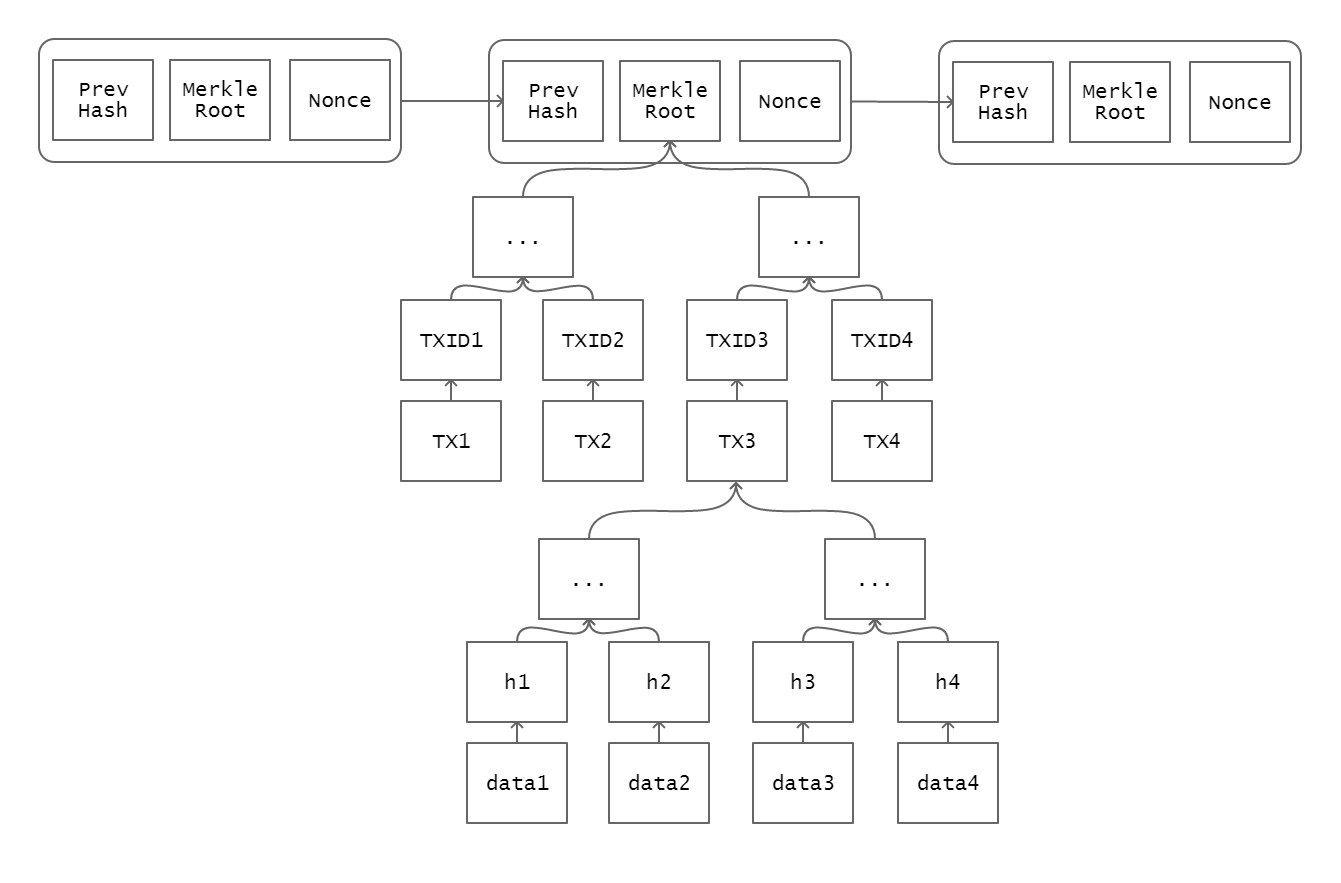
\includegraphics[width=\linewidth]{Images/bitcoin-chain-calendar.png}
		\caption[Calendar timestamping.]{Calendar timestamping. $TX_3$ is the transaction made by the calendar, it includes a commitment to $\{data_i\}_{i=1}^n$ obtained with a Merkle tree. Note that transaction must follow the consensus rules to be included in the chain, instead data are completely arbitrary.}
		\label{fig:chain-calendar}
	\end{center}
\end{figure}

A calendar spends its own bitcoin to do a transaction, this implies that he won't be able to perform an extremely high number of transactions, leading to less frequent timestamps. As of writing, the calendars use the \textit{replace by fee} (\textit{RBF}) mechanism to spend a fix amount of bitcoin each day. In Algorithm \ref{alg:calendar-rbf} is described a simplified scheme of its working.
This procedure makes the calendar expenditures fixed: each day has approximately 144 block, so the amount spent in fee per day is $144 \cdot a$, where $a$ is a fixed value set by who run the calendar.

Thus if the mean fee to get into the next block is high, then the calendar may wait several blocks before timestamping and clients will have to wait for a long time to have their receipt upgraded and their data timestamped. This issue can be addressed if someone is timestamping in place of the calendar, which could be facilitated by the technique we are showing in Chapter \ref{chpr:ec-commitments}. 

Despite all these considerations, the existence of public calendars is an extremely remarkable achievement for users: they enable clients to timestamp completely for free their own data. 
The solution involves some trust\footnote{Actually a client may implement a trustless system involving the calendar to timestamp his data. He would first ask the calendar to timestamp and then wait for the completed proofs; after a reasonable amount of time, if the calendar delivered what promised, then the client is fine, otherwise he timestamps by himself.}, but for a limited interval of time and with minimal possible downsides; once the proof is completed, it is not important if it was created through a central hub, it has the exact same respectability of any other proof. 
Furthermore the calendar learned nothing about the data timestamped since it received only an hash value. 
Ultimately the efficient aggregation reduces the burden caused to the network, making timestamping sustainable even on large scale.

\begin{algorithm}
	\caption{Calendar replace by fee}
	\label{alg:calendar-rbf}
	\begin{algorithmic}[1]
		\Procedure{calendarRBF}{$a,LT$}\Comment{step $a$, last timestamp $LT$}
		\State $fee \gets 0$
		\Repeat 
		\State $fee \gets fee + a$
		\State $S \gets \{h_i\}_{i=1}^n$ \Comment{collect clients timestamp requests}
		\State $MR \gets$ \Call{merklelize}{$S$}
		\State $TX \gets$ \Call{maketx}{$fee, MR$} \Comment{create transaction including $MR$}
		\State broacast $TX$
		\Until{$TX$ is mined}
		\State \textbf{return} $LT$ \Comment{$LT$ to restart the procedure}
		\EndProcedure
	\end{algorithmic}
\end{algorithm}